\documentclass{article}
\usepackage{scrextend}
\usepackage{mathrsfs}
\usepackage{amsmath}
\usepackage{amsthm}
\usepackage{amssymb}
\usepackage{graphicx}
\usepackage{subcaption}
\usepackage{color}
\usepackage{bm}
%\include{macros}
%\usepackage{floatflt}
%\usepackage{graphics}
%\usepackage{epsfig}


\theoremstyle{definition}
\newtheorem{theorem}{Theorem}[section]
\newtheorem{lemma}[theorem]{Lemma}
\newtheorem{proposition}[theorem]{Proposition}
\newtheorem{corollary}[theorem]{Corollary}

\theoremstyle{definition}
\newtheorem*{defition}{Definition}
\newtheorem*{example}{Example}

\theoremstyle{remark}
\newtheorem*{remark}{Remark}
\newtheorem*{note}{Note}
\newtheorem*{exercise}{Exercise}

\setlength{\oddsidemargin}{-0.25 in}
\setlength{\evensidemargin}{-0.25 in} \setlength{\topmargin}{-0.25
in} \setlength{\textwidth}{7 in} \setlength{\textheight}{8.5 in}
\setlength{\headsep}{0.25 in} \setlength{\parindent}{0 in}
\setlength{\parskip}{0.1 in}

\newcommand{\homework}[4]{
\pagestyle{myheadings} \thispagestyle{plain}
\newpage
\setcounter{page}{1} \setcounter{section}{#4} \noindent
\begin{center}
\framebox{ \vbox{\vspace{2mm} \hbox to 6.28in { {\bf
THU-70250043,~Pattern~Recognition~(Spring 2017) \hfill Homework: 1} }
\vspace{6mm} \hbox to 6.28in { {\Large \hfill #1 \hfill} }
\vspace{6mm} \hbox to 6.28in { {\it Lecturer: #2 \hfill} }
\vspace{2mm} \hbox to 6.28in { {\it Student: #3 \hfill} }
\vspace{2mm} } }
\end{center}
\markboth{#1}{#1} \vspace*{4mm} }


\begin{document}

\homework{Bayesian Methods}{Changshui Zhang
  \hspace{5mm} {\tt zcs@mail.tsinghua.edu.cn}}{Xuefei Ning \hspace{5mm} {\tt foxdoraame@gmail.com
 } }{8}

%%%%%%%%%%%%%%%%%%%%%%%%%%%%%%%%%%%%%%%%%%%%%%%%%%%%%%%%%%%%%%%%%%%%
% Section 2.  Problem
%%%%%%%%%%%%%%%%%%%%%%%%%%%%%%%%%%%%%%%%%%%%%%%%%%%%%%%%%%%%%%%%%%%%

1. \\
1.1.
\begin{addmargin}[3em]{2em}
The log likihood function of the samples $\{k_1, k_2, \dots, k_n\}$ is
\[
L(\{k_i\} | \lambda) = \ln(\prod_{i=1}^n \frac{\lambda^{k_i} \exp(-\lambda)}{k_i!}) = \sum_{i=1}^n (k_i \ln(\lambda) - \lambda - \ln(k_i!))
\]
Calculate the derivative with respect to $\lambda$, we get:
\[
\frac{\partial L}{\partial \lambda} = \sum_{i=1}^n \frac{k_i}{\lambda} - 1 = \frac{\sum_{i=1}^N k_i}{\lambda} - n
\]
And we can see that the second derivative of the log likelihood function is always negative as $\lambda > 0$, so this function is a concave function, and the maximum of this function is achieved at its unique extreme point, so at the extreme point we have:
\[
\frac{\sum_{i=1}^N k_i}{\lambda} - n = 0 \leadsto \lambda_{mle} = \frac{\sum_{i=1}^N k_i}{n}
\]
\end{addmargin}

1.2.
\begin{addmargin}[3em]{2em}
  \[
  E[K] = \sum_{k=0}^{\infty} \frac{\lambda^k \exp(-\lambda)}{k!} k = \sum_{k=1}^{\infty} \lambda \frac{\lambda^{k-1} \exp(-\lambda)}{(k-1)!} = \lambda \sum_{k'=0}^{\infty} \frac{\lambda^{k'} \exp(-\lambda)}{k'!} = \lambda
  \]
  \[
  \begin{split}
    Var[K] & = E[K^2] - {E[K]}^2 = \sum_{k=0}^{\infty} \frac{\lambda^k \exp(-\lambda)}{k!} k((k-1) + 1) - \lambda^2 \\
    & = \sum_{k=0}^{\infty} \frac{\lambda^k \exp(-\lambda)}{k!} k(k-1) + E[K] - {E[K]}^2 \\
    & = \lambda^2 \sum_{k'=0}^{\infty} \frac{\lambda^{k'} \exp(-\lambda)}{k'!} + E[K] - {E[K]}^2 \\
    & = \lambda^2 + \lambda - \lambda^2 = \lambda
  \end{split}
  \]

The expectation and variance of $\lambda_{mle}$ is:
\[
E[\lambda_{mle}] = \frac{1}{n} \sum_{i=1}^n E(k_i) = E(k_i) = \lambda
\]

\[
Var[\lambda_{mle}] = E(\lambda_{mle}^2) - {E(\lambda_{mle})}^2 = \frac{nE(K^2) + (n^2 - n)E(K)^2}{n^2} -\lambda^2 = \frac{\lambda}{n}
\]
From the two results above, we can see the $\lambda_{mle}$ is the unbiased estimation of $\lambda$. And as the number of samples increase, the variance of the estimation decreases, the estimation is more accurate, so this estimation is a effective estimation of $\lambda$.
\end{addmargin}

1.3.

\begin{addmargin}[3em]{2em}
  The posterior probability of $\lambda$ is:
  \[
  P(\lambda | \{k_i\}) = \frac{L(\{k_i\} | \lambda) p(\lambda)}{P(\{k_i\})}
  \]
  In which $P(\{k_i\})$ is the evidence of the observed samples $\{k_i\}$ intergrated on all the possible value of the parameter $\lambda$, the parameter $\lambda$ is marginalized out, so it is unrelated to $\lambda$. We take the logarithm of of the above equation, get:
  \[
  \begin{split}
  \log(P(\lambda | \{k_i\})) = \sum_{i=1}^N (k_i \ln(\lambda) - \lambda - \ln(k_i!)) + \ln(p(\lambda)) - \ln(P(\{k_i\})) \\
  = \sum_{i=1}^N (k_i \ln(\lambda) - \lambda - \ln(k_i!)) + (a-1)\ln(\lambda) - \frac{\lambda}{\beta} - \ln(\Gamma(a)) - a \ln(\beta)
  \end{split}
  \]
  Take the derivative and make it equal to 0:
  \[
  \begin{split}
  \frac{\partial P(\lambda | \{k_i\})}{\lambda} = \frac{\sum_{i=1}^N + a - 1}{\lambda} - (1 + \frac{1}{\beta}) = 0 \\
  \leadsto \lambda_{map} = \frac{a - 1 + \sum_{i=1}^n k_i}{n + \frac{1}{\beta}}
  \end{split}
  \]

\end{addmargin}

1.4.

\begin{addmargin}[3em]{2em}
  \begin{itemize}
  \item When $n \rightarrow 0$, $\lambda_{map} \rightarrow (a-1)\beta$, this is the mode value of the prior gamma distribution (the value with the maximum prior).
  \item When $n \rightarrow \infty$, $\lambda_{map} \rightarrow \frac{\sum_{i=1}^n k_i}{n}$, this is the maximum-likelihood estimation of $\lambda$: $\lambda_{mle}$.
  \end{itemize}
  \quad We can see from the two limiting case: when there are few samples, the prior distribution contributes much to the MAP estimation; while as the number of samples increase, the effect of the prior distribution fades out, and the actual samples contributes more to the MAP estimation, which will drive the MAP estimation to $\lambda_{mle}$.\\

  \quad Also, we can notice that the gamma distribution $\mbox{Gamma}(a, \beta)$ is the \textit{conjugate prior} of the poison likelihood function: the posterior distribution of $\lambda$ is of the same distribution family as the prior (both Gamma distribution). So the sample-adding process can be regard as an progressively parameter adjusting process of the gamma distribution (adding a new sample just ajust $a$ and $\beta$ a little). This perspective will make the MAP estimation easy to calculate progressively(at every step, the last posterior distribution can be regard as a new prior), and unrelated to the exact number of samples $n$ that have been observed.

\end{addmargin}

2.\\
2.1.

\begin{addmargin}[3em]{2em}
  The log likelihood function is:
    \[
  \begin{split}
    L(X) = P(\{x_1, \dots, x_n\} | \mu, \Lambda^{-1}) & = \prod_{i=1}^{n} P(x_i | \mu, \Lambda) \\
    & = \prod_{i=1}^{n} \frac{1}{\sqrt{{(2\pi)}^p|\Lambda^{-1}|}} \exp(-\frac{1}{2} {(x_i - \mu)}^T \Lambda (x_i - \mu))\\
    & = \frac{1}{{(2\pi)}^{\frac{pn}{2}}} {\Lambda}^{\frac{n}{2}} \exp(-\frac{1}{2} \sum_{i=1}^n {(x_i - \mu)}^T \Lambda (x_i - \mu)) \\
    \mbox{logL}(X) = \log(L(X)) & = \frac{n}{2} \log(|\Lambda|) - \frac{pn}{2} \log(2\pi) - \frac{1}{2} \sum_{i=1}^n {(x_i - \mu)}^T \Lambda (x_i - \mu)
  \end{split}
  \]
  To do the MLE estimation of $\mu$, we take the partial derivative:
  \[
  \frac{\partial \mbox{logL(X)}}{\partial \mu} = \sum_{i=1}^n \Lambda (x_i - \mu) = \Lambda \sum_{i=1}^n (x_i - \mu) = 0  \]
  As $\Lambda^{-1}$ is non-singular, its null space is empty set. So, we must have:
  \[
  \sum_{i=1}^n (x_i - \mu) = 0 \leadsto \mu_{mle} = \frac{1}{n} \sum_{i=1}^n x_i
  \]
  To do the MLE estimation of $\Lambda$, we take the partial derivative:
  \[
  \frac{\partial \mbox{logL(X)}}{\partial \Lambda} = \frac{n}{2} \Lambda^{-T} - \frac{1}{2} \sum_{i=1}^n (x_i - \mu)(x_i - \mu)^T = 0
  \]
  As $\Lambda$ is non-singular and symmetric, we get:
  \[
  \Lambda_{mle} = {(\frac{1}{n} \sum_{i=1}^n (x_i - \mu_{mle}){(x_i - \mu_{mle})}^T)}^{-1}
  \]
\end{addmargin}

2.2.

\begin{addmargin}[3em]{2em}
  The log posterior function is:
  \[
  \begin{split}
    \log(L(X)) & + \log(gw(\mu, \Lambda)) - \log(P(X))\\
    & = C + \frac{v-p+n}{2}\ln(|\Lambda|) - \frac{1}{2} \sum_{i=1}{n} (x_i - \mu)^T \Lambda (x_i - \mu) - \frac{1}{2}s(\mu - \mu_0)^T \Lambda (\mu - \mu_0) - \frac{\mbox{tr}(V^{-1}\Lambda)}{2}
  \end{split}
  \]
  $C$ is a constant that do not influence the deriviative. The MAP estimation of $\mu$ satisify:
  \[
  \frac{\partial \mbox{posterior}}{\partial \mu} = \sum_{i=1}^n \Lambda (x_i - \mu) - s \Lambda (\mu - \mu_0) = \Lambda (\sum_{i=1}^n x_i + s\mu_0 - (n+s)\mu) = 0
  \]
  As $\Lambda$ is non-singular, we have $\mu_{map} = \frac{\sum_{i=1}^n x_i + s\mu_0}{n + s}$.
  The MAP estimation of $\Lambda$ statisfy:
  \[
  \frac{\partial \mbox{posterior}}{\partial \Lambda} = \frac{v - p + n}{2}\Lambda^{-T} - \frac{1}{2} \sum_{i=1}^n (x_i - \mu)(x_i - \mu)^T - \frac{1}{2} s (\mu - \mu_0)(\mu - \mu_0)^T - \frac{V^{-T}}{2} = 0
  \]
  Substitute in $\mu_{map}$, we get:
  \[
  \Lambda_{map} = {(\frac{\sum_{i=1}^n (x_i - \mu_{map}){(x_i - \mu_{map})}^T + s(\mu_{map} - \mu_0) (\mu_{map} - \mu_0)^T + V^{-T}}{n + v - p})}^{-1}
  \]

\end{addmargin}

2.3.
\begin{addmargin}[3em]{2em}
  \begin{itemize}
  \item When $n \rightarrow 0$, $\mu_{map} \rightarrow \mu_0$; $\Lambda_{map} \rightarrow \frac{V}{v-p}$.
  \item When $n \rightarrow \infty$, $n >> s, \mu_{map} \rightarrow \frac{\sum_{i=1}^n x_i}{n} = \mu_{mle}$; substitute $\mu_{map}$ into $\Lambda_{map}$, also use $n>>s$, we have$\Lambda_{map} \rightarrow \Lambda_{mle}$.
  \end{itemize}
      Very intuitively, when there are few samples, the piror distribution of $\mu$ and $\Lambda$ contributes much to the posterior distribution, so when $n = 0$, the MAP estimation is just the mode value of the prior distribution of the parameters. However, as $n$ increases, the samples $\{x_i\}$ contribute more and more to the posterior distribution, and when $n \rightarrow \infty$, the influence of the prior distribution fades out, so the MAP estimation when $n \rightarrow \infty$ will approach the MLE estimation where parameter prior is not used.\\

      Also, the Gaussian-Wishart prior is the conjugate prior distribution of the Gaussian likelihood function, so we can see the sample-adding process as a progressively ajustment process of the hyper-parameters $V, v, s, \mu_0$ to get the posterior distribution. This property leads to quicker and simpler posterior calculation and hence MAP estimation.
\end{addmargin}

3.\\
3.1.

% http://stats.stackexchange.com/questions/133347/ml-estimate-of-exponential-distribution-with-censored-data
% http://www.itl.nist.gov/div898/handbook/apr/section4/apr412.htm
\begin{addmargin}[3em]{2em}
  Suppose we have a failure model of a certian type of device, we use exponential distribution to model the failure process of this type of device ($F_{\mbox{failure}}(t) = P(\mbox{failure\_time} <= t) = 1 - \exp(-\lambda t)$), in which the failure rate of this type of device remains unchanged during the lifetime of the device:
  \[
  \lambda(t) = \frac{f(t)}{1 - F(t)} = \lambda
  \]
    Suppose we observe the behavior of $N$ such devices for a period: $T$. We assume in this time period, there are $n$ device failure observed, we assume the $n$ devices failed at $t_1, t_2, \dots, t_n$. We can write the likelihood function of these observation as:
  \[
  \mbox{logL} = \log(\prod_{i=1}^n \lambda \exp(-\lambda t_i) {(1-F(T))}^{N-n}) = n \ln(\lambda) - \lambda \sum_{i=1}^n t_i - (N-n) \lambda T
  \]
  When $n = 0$, the log likelihood function is:
  \[
  \mbox{logL}(\lambda) = - N \lambda T
  \]
  The maximum is achieved at $\lambda = 0$, however, $\lambda = 0$ does not correspond to a legal exponential distribution, because every exact point have a probability of 0. So, in this situation, the MLE estimation do not exist.
\end{addmargin}

3.2.

\begin{addmargin}[3em]{2em}
  Consider a mixture of two fixed-mean fixed-variance gaussian distribution with the same $\Sigma$, the parameter $\theta, 0 \leq \theta \leq 1$ is the combination factor of the two gaussian probabilistic function:
  \[
  p(x | \theta) = \theta \frac{1}{{(2\pi)}^{n/2}|\Sigma^{-1}|} \exp(-\frac{(x - \mu_1)^T \Sigma^{-1} (x - \mu_1)}{2}) + (1 - \theta) \frac{1}{{(2\pi)}^{n/2}|\Sigma^{-1}|} \exp(-\frac{{(x - \mu_2)}^T \Sigma^{-1} (x - \mu_2)}{2})
  \]

  When the observed sample $x_s$ is at the middle point of $\mu_1$ and $\mu_2$, that is $x_s = \frac{\mu_1 + \mu_2}{2}$, the MLE of the parameter $\theta$ is not unique, because $\theta$ can be every value in $[0, 1]$, and the likelihood of this special sample won't change.

\end{addmargin}

3.3.

\begin{addmargin}[3em]{2em}
  To guarantee the MLE of parameter always exists and its uniqueness, the log likelihood function should have the only maximum point no matter what samples are observed.
\end{addmargin}

4.\\
4.1.
\begin{addmargin}[3em]{2em}
  The log likelihood of the observation $T=\{t_i\}$ is:
  \[
  \log(p(T | X, \omega, \beta)) = -N \ln(\frac{2 \pi}{\sqrt{\beta}}) - \frac{\beta}{2} \sum_{i=1}^N {(t - y(x, \omega))}^2
  \]
  In maximum likelihood estimation, we maximize the log likelihood function, which is to minimize $\sum_{i=1}^N {(t - y(x, \omega))}^2$ according to the equation above. So this is equivalent to minimizing the sum of square error.
\end{addmargin}

4.2.

\begin{addmargin}[3em]{2em}
  \[
  \log(p(\omega)) \propto \log(p(T | X, \omega, \beta)) + \log(p(\omega | \alpha)) = C - \frac{\beta}{2} \sum_{i=1}^N {(t - y(x, \omega))}^2 - \alpha \frac{\omega^T \omega}{2}
  \]
  Doing the MAP estimation of the posterior distribution of $\omega$, is equivalent to minimize $\frac{\beta}{2} \sum_{i=1}^N {(t - y(x, \omega))}^2 + \alpha \frac{\|\omega\|}{2}$, this is the form of the square error loss with a weight decay regularizing term (when $\alpha = \beta$).
\end{addmargin}

\section*{Naive Bayes}

1.\\

\begin{addmargin}[3em]{2em}
  When $Y = T$, we need a parameter $P(X_1 = T | Y = T)$ for $X_1$, and two parameter $\mu_i, \sigma_i$ for every other continous variable $X_i$. And another set of parameters are needed when $Y = F$. So we need $2(1 + 2(n-1)) = 2(2n-1)$ parameters to build the Naive Bayes classifier.\\

  \[
  P(Y=y|X) = \frac{P(X|Y)P(Y)}{P(X)} = \frac{P(X_1|Y=y) \prod_{i=2}^n P(X_i|Y) P(Y)}{P(X_1|Y=T) \prod_{i=2}^n P(X_i|Y=T) + P(X_1|Y=F) \prod_{i=2}^n P(X_i|Y=F) }
  \]
  In the above equation, $P(Y)$ prior is estimated using the occuring times of $Y=T$ and $Y=F$ in the training data.
\end{addmargin}

2.\\
2.1.
\begin{addmargin}[3em]{2em}
  We use $S$ for the abbreviation of the random variable $Sunny$, $W$ for $Windy$ and $H$ for $Hike$. The posterior distribution of $H$ is:
  \[
  P(H | S, W) = \frac{P(S, W | H)P(H)}{P(S, W, H)} = \frac{P(S | H)P(W | H)P(H)}{P(S|H=T)P(W | H = T)P(H=T) + P(S|H=F)P(W | H = F)P(H=F)}
  \]
  The decision rule is:
  \[
  \begin{cases}
    \hat{H}=T: P(H=T|S,W) > P(H=F|S,W) \leadsto P(S|H=T)P(W|H=T) > P(S|H=F)P(W|H=F)\\
    \hat{H}=F: \mbox{otherwise}
  \end{cases}
  \]
  The four cases is listed below:
  \begin{itemize}
  \item $S=T, W=T$, $0.27 = P(S=T|H=T)P(W=T|H=T) < P(S=T|H=F)P(W=T|H=F) = 0.32$, so the decision is $\hat{H} = F$.
  \item $S=T, W=F$, $0.63 = P(S=T|H=T)P(W=F|H=T) > P(S=T|H=F)P(W=F|H=F) = 0.08$, so the decision is $\hat{H} = T$.
  \item $S=F, W=T$, $0.03 = P(S=F|H=T)P(W=T|H=T) < P(S=F|H=F)P(W=T|H=F) = 0.48$, so the decision is $\hat{H} = F$.
  \item $S=F, W=F$, $0.07 = P(S=F|H=T)P(W=F|H=T) > P(S=F|H=F)P(W=F|H=F) = 0.12$, so the decision is $\hat{H} = F$.
  \end{itemize}
\end{addmargin}

2.2.
\begin{addmargin}[3em]{2em}
  \[
  \begin{split}
    P(\mbox{error}) = & \sum_{s, w \mbox{ s.t. } \hat{H}=T}P(H=F|S=s,W=w)P(S=s, W=w)\\
    & + \sum_{s, w \mbox{ s.t. } \hat{H} = F}P(H=T|S=s, W=w)P(S=s, W=w) \\
    = & \sum_{s, w \mbox{ s.t. } \hat{H}=T}P(S=s,W=w|H=F)P(H=F)\\
    & + \sum_{s, w \mbox{ s.t. } \hat{H}=F}P(S=s,W=w|H=T)P(H=T) \\
    = & 0.08 * 0.5 + (0.27 + 0.03 + 0.07) * 0.5 = 0.225
  \end{split}
  \]
\end{addmargin}

2.3.
\begin{addmargin}[3em]{2em}
   The joint probability is:
\[
P(S=T,W=T,H=T) = P(H=T)p(S=T|H=T)P(W=T|H=T) = 0.135
\]
\end{addmargin}

2.4.

\begin{addmargin}[3em]{2em}
  The naive bayes assumption is violated, because the $\mbox{Sunny}$ random variable is dependent to $\mbox{Rainy}$ variable even if the decision is given. The joint probability remains unchange here:
  \[
  P(S=T,W=T,H=T) = P(H=T)p(S=T|H=T)P(W=T|H=T) = 0.135
  \]
\end{addmargin}

2.5.
\begin{addmargin}[3em]{2em}
  The error rate remains unchanged as $0.225$, and the performance of Naive Bayes does not improve by observing the new attribute Rainy, because $\mbox{Rainy} = \neg \mbox{Sunny}$, and it brough no additional information.
\end{addmargin}


\section*{Programming}
In this problem you will implement Naive Bayes and Logistic Regression, then compare their performance on a
document classification task. The data for this task is taken from the 20 Newsgroups data set, and is available
from the attached zip file. The included README.txt describes the data set and file format.

Our Naive Bayes model will use the bag-of-words assumption. This model assumes that each word in a
document is drawn independently from a multinomial distribution over possible words. (A multinomial
distribution is a generalization of a Bernoulli distribution to multiple values.) Although this model ignores
the ordering of words in a document, it works surprisingly well for a number of tasks. We number the words
in our vocabulary from 1 to $m$, where $m$ is the total number of distinct words in all of the documents.
Documents from class $y$ are drawn from a class-specific multinomial distribution parameterized by $\theta_y$. $\theta_y$ is
a vector, where $\theta_{y,i}$ is the probability of drawing word $i$ and $\sum_{i=1}^m \theta_{y,i}=1$.
Therefore, the class-conditional probability of drawing document x from our Naive Bayes model is
$P(X = x|Y = y) = \prod_{i=1}^m (\theta_{y,i})^{count_i(x)}$, where $count_i(x)$ is the number of times word $i$ appears in $x$.

1. Provide high-level descriptions of the Naive Bayes and Logistic Regression algorithms. Be
sure to describe how to estimate the model parameters and how to classify a new example.

\begin{addmargin}[3em]{2em}
  \textbf{Naive Bayes Classifier}
  For Naive Bayes Classifier, we learn the generative model of the documents by learning $P(Y)$ and $P(X|Y)$. The likelihood function $P(X|Y)$ can be factorized as $P(X = x|Y = y) = \prod_{i=1}^m (\theta_{y,i})^{count_i(x)}$ from the bag-of-word assumption; The prior distribution of document labels $Y$ can be easily modelsed using the normalized count of the occurence of $Y=y$ in the training data.\\
  Assume there are $M_y$ samples for every document label $y$:
  \[
  P(Y = y) = \frac{M_y}{\sum_{i} M_i}
  \]
  In the learning process, we want to obtain the MLE estimation of the parameter $\{\theta{y, i} i=1,\dots, m\}$ set for every document label $y$. Assume there are $N$ samples that are labeled $y$ in the training data, we can write the log likelihood function:
  \[
  \ln(\prod_{n=1}^N P(X | Y=y)) = \sum_{n=1}^N \sum_{i=1}^m count_i(x^{(n)}) \ln(\theta_{y,i})
  \]
  Also, there is a constraint for $\theta_{y,i}$ that $\sum_{i=1}^{m} \theta_{y, i} = 1$. We can obtain the Lagrangian of this problem:
  \[
  \sum_{n=1}^N (\sum_{i=1}^m count_i(x^{(n)}) \ln(\theta_{y,i})) - a(\sum_{i=1}^m \theta{y, i})
  \]
  Take the derivative with respect to $\theta_{y, i}$, we have:
  \[
  \begin{split}
    & \frac{\sum_{n=1}^N count_i(x^{(n)})}{\theta_{y, i}} - a = 0\\
    & \leadsto \theta_{y_i} \propto \sum_{n=1}^N count_i(x^{(n)})\\
    & \leadsto \theta_{y_i} = \frac{\sum_{n=1}^N count_i(x^{(n)})}{\sum_{i=1}^m \sum_{n=1}^N count_i(x^{(n)})}
  \end{split}
  \]

  From the above estimation equation, we can see that we just need to count the occurence of words $i$ in samples grouped by the label $y$, after which the parameters can be obtained by doing some normalization.\\

  In the test phase, we get a test sample $x$, we should calculate $P(X=x|Y=y)P(Y=y)$ for every $y$ (The evidence term $P(X=x)$ is ignored in the posterior as it's the same for every $y$). And take the $y$ that maximise $P(X=x|Y=y)P(Y=y)$ as the classification result.\\

  \textbf{Logistic Regression}
  Here, we are using logsitic regression for multi-class classification, in which the logistic regression can also be called Softmax Regression. It is a discriminative model that directly model the conditional/posterior distribution $P(Y=y|X=x)$ instead of the joint distribution. The model is parameterized as follow:
  \[
  P(Y = y | X = x; \theta) = \frac{\exp(\theta_y^\top x)}{\sum_{j=1}^K \exp(\theta_j^{\top} x)}
  \]
  We take the logarithm of the likelyhood of all the training data, and we can get:
  \[
  J = \ln(\prod_{n=1}^N P(y^{(n)}|x^{(n)}; \theta)) = \sum_{n=1}^N (\theta_{y^{(n)}}^{\top} x^{(i)} - \ln(\sum_{j=1}^K \exp(\theta_j^{\top} x)))
  \]
  Take the derivative with respect to the parameter vector $\theta_k$, we get:
  \[
  \nabla_{\theta_k} J = \sum_{n=1}^N (I(y = k) - \frac{\exp(\theta_k^{\top} x)}{\sum_{j=1}^K \exp(\theta_j^{\top} x)}) x
  \]
  In the above equation, $I(\bullet)$ is the indicator function that is 1 when the condition is true otherwise 0.\\
  However, a closed-form solution cannot be found that make this derviative equals to 0. So we can use a local optimization method such as gradient descent or its variants to solve this problem.

  In GD, the update of parameters follows:
  \[
  \theta_k \leftarrow \theta_k - a \nabla_{\theta_k} J
  \]
  Also, we can consider using SGD or adding regularization, momentum.\\

  In the test phase, we get a test sample $x$, we calculate $\exp(\theta_y^{\top} x)$ for every $y$, and take the $y$ that miximise that value as the classification result.
\end{addmargin}

2. Imagine that a certain word is never observed in the training data, but occurs in a test
instance. What will happen when our Naive Bayes classifier predicts the probability of the this test
instance? Explain why this situation is undesirable. How to avoid this problem? Will logistic regression have a similar problem?
Why or why not?

\begin{addmargin}[3em]{2em}
  In Naive Bayse method, if we just make the likelihood of words given document label $y$ that did not occur in the training data labeled $y$ to be 0, once such a word occurs in one training data, the posterior probability of the document label being $y$ will be 0. This situation is certainly undesirable, because there are so many words that may be not included in a relatively small training set. Also, we can considier that when there is a test sample with a word with id $i$ that never occur in any training samples, then the posterior probability for all $y$ given this sample is 0. \\
  So, we can use a method that is analogous to ridge estimation in which a bias of estimation is introduced to guarantee numerical stability (to smooth the problem) -- we can add one to the count of every words so that no likelihood of one word will be 0. We do not need to do the add-one smoothing explicitly, this procedure should be done lazily when testing for effiency, because this problem has a very sparse but large input space.\\
  As for logistic regression, there might also be some word that do not occur in any of the training data -- for example, in the test data, there is a word id `61188' that is bigger than any other word ids in the training data. So in this situation, we should ignore the word count of this word $j$ (it's equivalent as the weight of this word $j$ satisify: $\theta_{ij} = 0$ for all document labels $i$).

\end{addmargin}

3. Implement Logistic Regression and Naive Bayes. Use add-one smoothing when estimating
the parameters of your Naive Bayes classifier. For logistic regression, we found that a step size around
0.0001 worked well. Train both models on the provided training data and predict the labels of the test
data. Report the training and test error of both models. Submit your code along with your homework.

\begin{addmargin}[3em]{2em}
  \begin{center}
    \begin{tabular}{ | c | c | c | }
      \hline
      Model & Train Error & Test Error\\\hline
      Naive Bayes & 5.67\% & 21.48\%\\
      Logistic Regression-exp1 (20 epoch) & 40.26\% & 50.53\%\\
      Logistic Regression-exp2 (20 epoch) & - & 49.29\%\\
      Logistic Regression-exp2 (40 epoch) & 35.22\% & 46.60\% \\
      Logistic Regression-exp3 (SGD 20 epoch) & \% & 40.71\% \\

      \hline
    \end{tabular}
  \end{center}
  Some screenshots is shown below:
  \begin{figure}
    \centering%
    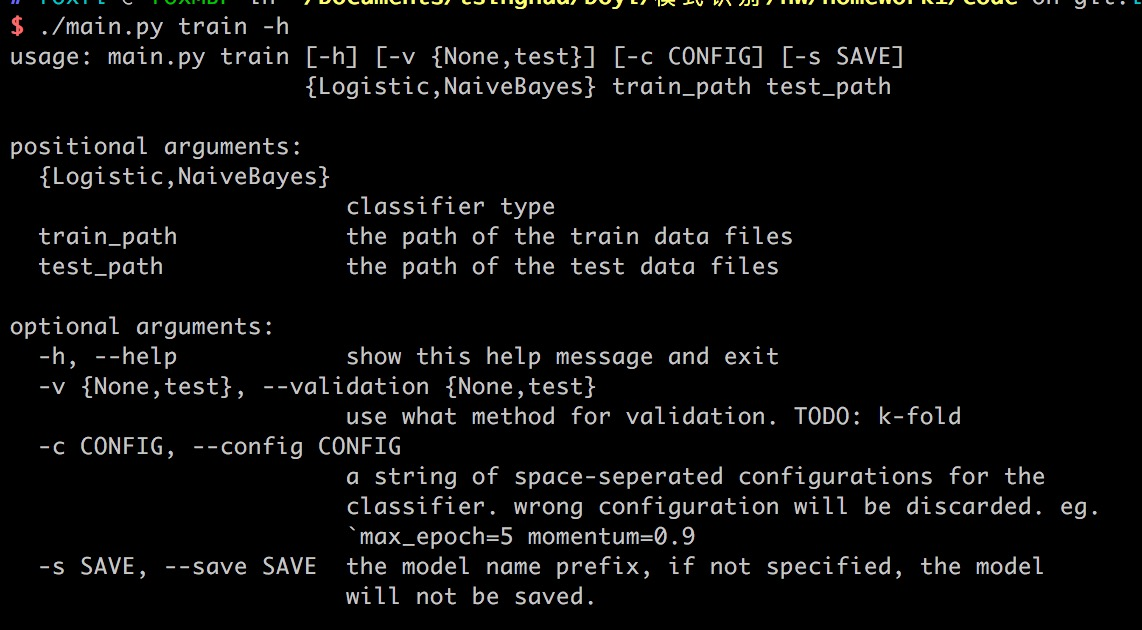
\includegraphics[height=5cm]{help.jpeg}
    \caption{View The Help Message}
  \end{figure}

  \begin{figure}
    \centering%
    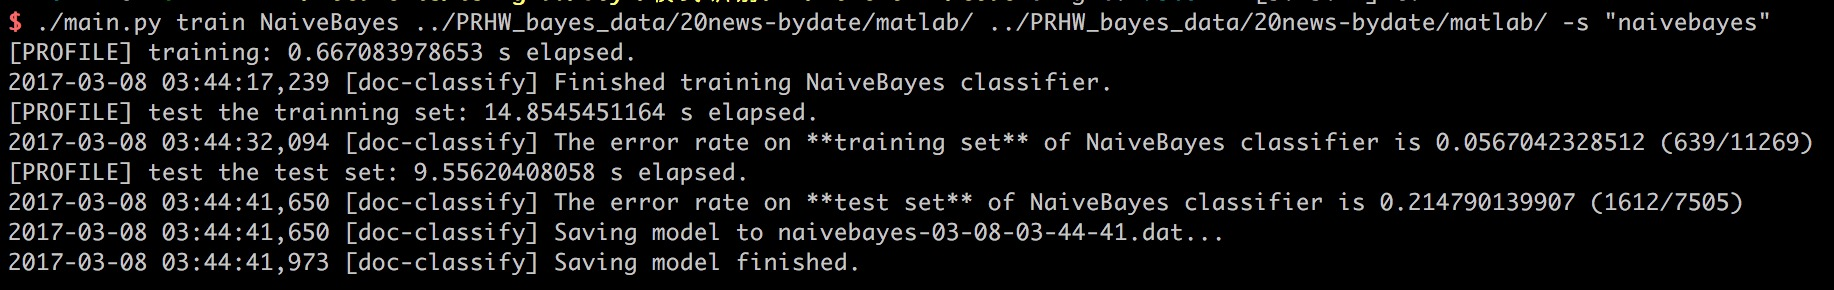
\includegraphics[height=3cm]{nb_run.jpeg}
    \caption{Naive Bayes Training}
  \end{figure}

  \begin{figure}[!tbp]
    \centering%
    \begin{subfigure}[b]{\columnwidth}
      \centering
      \includegraphics[height=1cm]{lr_run11.jpeg}
    \end{subfigure}

    \vspace{2em}

    \begin{subfigure}[b]{\columnwidth}
      \centering
      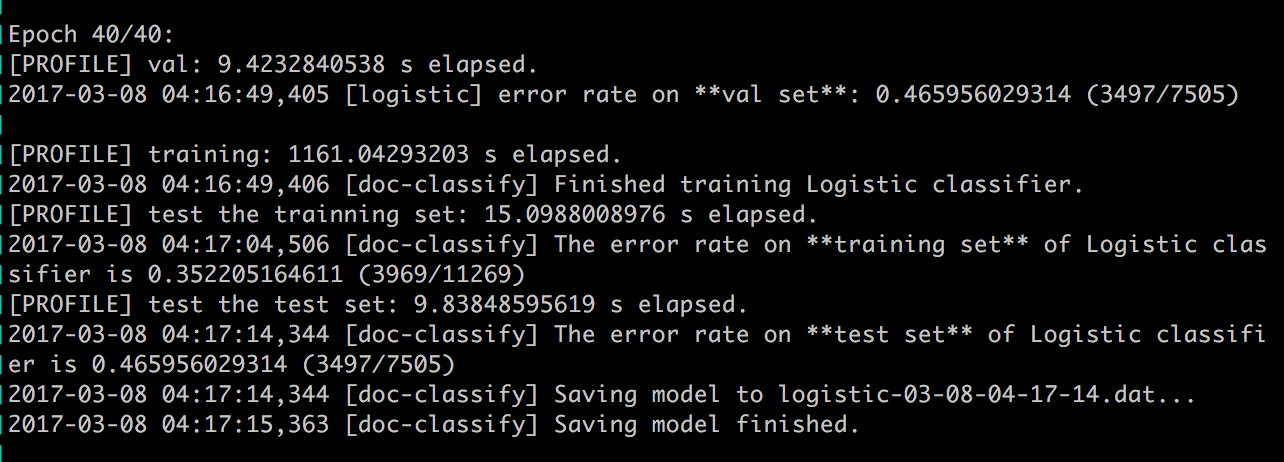
\includegraphics[height=4cm]{lr_run2.jpeg}
    \end{subfigure}

    %% \subcaptionbox{}[3cm]
    %% {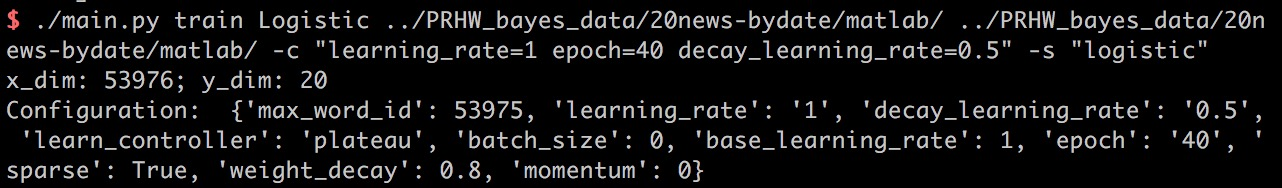
\includegraphics[height=2cm]{lr_run1.jpeg}}
    %% \hspace{3em}%
    %% \subcaptionbox{}[3cm]
    %% {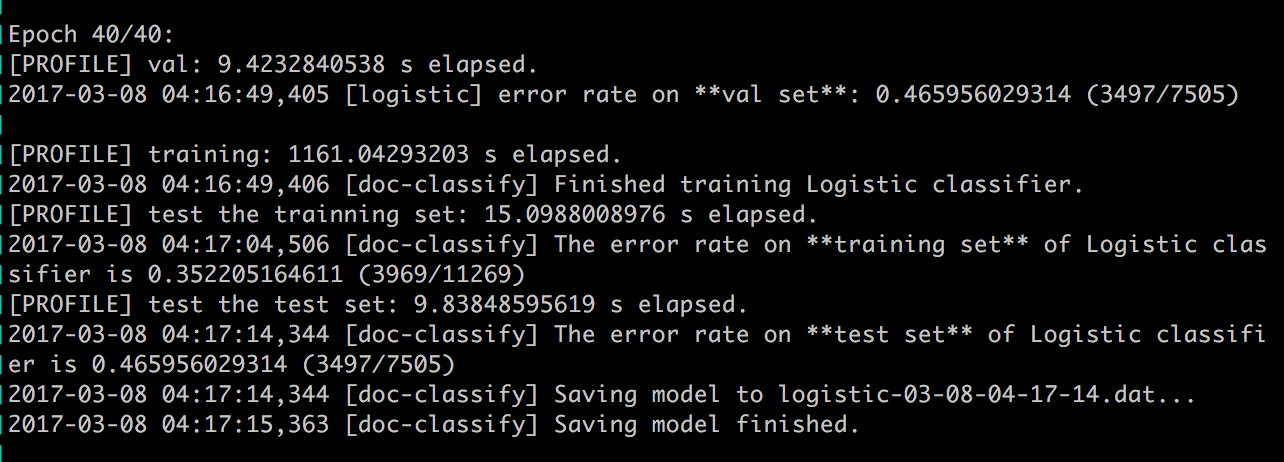
\includegraphics[height=2cm]{lr_run2.jpeg}}
    \caption{Logistic Regression Training of exp2}
  \end{figure}

  In the experiement, I find that randomized parameter initialization will outperforms 0-initialization in Logistic Regression when the learning rate is small (If learning rate is sufficiently large, the randomized parameter initialization contribute very little after a few steps). The experiement showed that the randomness would influence the convergence speed of Logistic Regression. And the experiement results showed that there would still be imaprovement with more training epochs, as no plateau of error rate ss achieved in the two experiement: they all ended because the number of epochs exceeds the pre-defined limit (20/40).\\

  The hyper-parameters of non-stochastic GD are hard to tune... I tried for a while and give up trying any more. The ``0.0001'' learning rate does not work well in my case.\\

  SGD outperforms GD, the error rate of SGD training decreases faster.

  The entrance of this program is ``main.py'', and the usage of this scripts can be viewed using ``--help'' option. There are two subcommand ``train'' and ``test'' of which the detailed help message can also be viewd. This program has a dependency on the ``numpy'' lib for just using some basic matrix multiply and element-wise operation (When I'm coding the Naive Bayes classifier, I tried to keep the compatibility of this project for the situation that ``numpy'' is not installed. However, I get tired to write a counterpart and adapter for ``numpy.ndarray'', so the logistic part of program assumes the installation of ``numpy''). On my Mac OS X, the ``numpy'' version is ``1.10.0'', but any version with compatible basic matrix operation will do.\\

  \textbf{NOTE}: Altough the tool will print out several configurations like $\mbox{weight\_decay}$, $\mbox{momentum}$, I just tried some of them while debugging, but in the submitting code, code for some of the configurations are deleted or untested. Anyway, the default configuration (do not specify ``-c'' option) will work. And there are many ``FIXME'' and ``TODO'' in the code as this code is finished in a rush. Apologize... \\


\end{addmargin}

4. Which model performs better on this task? Why do you think this is the case?

\begin{addmargin}[3em]{2em}
  In my experiements, the Naive Bayes classifier performs better on this task. I think the reasons might come from several aspects including problem properties and model properties:
  \begin{itemize}
  \item Indepence Assumption: In the Naive Bayes classifier, we make the independence assumption between the occurence of different words when the document label $y$ is given. Although this assumption seems quite naive and unreal, the actual mutual information of most pair of words is small. So this assumption is practical, and can lead to simple learning process.
  \item Generative vs. Discriminateive: In this problem, as we said in \textbf{Indepence Assumption}, the actual way of how the world work is modeled by the bag-of-words assumption, and we think this assumption is reasonable and somehow practical, so a generative model that \textit{utilize the useful prior knowledge in this domain (modeling of the world)} has the potential to perform better.
  \item Sparse input space: This problem have a large but sparse input space, Logistic Regression will spend more effort learning unimportant weight than Naive Bayes. Also, because of the sparsity, Naive Bayes model eploits the sparsity better, and hence have less parameters than Logstic Regression, this helps avoiding overfit.
  \item Tunning difficulty: There are quite a few hyper-parameters to tune in Logistic Regression, it's hard and time-consuming to find a good hyper-parameters set. Conversly, the Naive Bayes barely need tunning to achieve a fairly good result.
  \end{itemize}
\end{addmargin}


%%%%%%%%%%%%%%%%%%%%%%%%%%%%%%%%%%%%%%%%%%%%%%%%%%%%%%%%%%%%%%%%%%%%
% Reference
%%%%%%%%%%%%%%%%%%%%%%%%%%%%%%%%%%%%%%%%%%%%%%%%%%%%%%%%%%%%%%%%%%%%
%\begin{thebibliography}{1}

%\bibitem{BoydVandenberghe2004}
%S. Boyd and L. Vandenberghe, \emph{Convex Optimization}, Cambridge
%University Press, 2004.

%\end{thebibliography}
\end{document}
